\documentclass[11pt,a4paper]{article}

% ---------- Packages ----------
\usepackage[a4paper,margin=2.5cm,headheight=14pt]{geometry}
\usepackage{microtype}
\usepackage{amsmath,amssymb}
\usepackage{graphicx}
\usepackage{subcaption}
\usepackage{booktabs,array,tabularx}
\usepackage{xcolor}
\usepackage{enumitem}
\usepackage{fancyhdr}
\usepackage{titlesec}
\usepackage{tcolorbox}
\usepackage{tikz}
\usetikzlibrary{arrows.meta,positioning,calc}
\usepackage[hidelinks]{hyperref}
\usepackage{float}
\usepackage{setspace}

% ---------- Colours ----------
\definecolor{navy}{HTML}{1F3A5F}
\definecolor{accent}{HTML}{D9731A}
\definecolor{good}{HTML}{2E8B57}
\definecolor{softgray}{HTML}{F3F5F8}

% ---------- Helpers ----------
\DeclareRobustCommand{\code}[1]{\texttt{\detokenize{#1}}}
\newcommand{\E}{\mathbb{E}}
\newcommand{\Var}{\operatorname{Var}}
\newcommand{\best}[1]{\textbf{\textcolor{good}{#1}}}

\setstretch{1.08}
\setlength{\parskip}{4pt}
\setlength{\parindent}{0pt}

% ---------- Section style ----------
\titleformat{\section}{\Large\bfseries\color{navy}}{\thesection}{0.7em}{}[\vspace{-0.4em}\color{navy}\titlerule]
\titleformat{\subsection}{\large\bfseries\color{navy}}{\thesubsection}{0.6em}{}
\titleformat{\subsubsection}{\normalsize\bfseries\color{navy}}{\thesubsubsection}{0.6em}{}
\titlespacing*{\section}{0pt}{16pt}{8pt}

% ---------- Header / footer ----------
\pagestyle{fancy}
\fancyhf{}
\fancyhead[L]{\small\color{gray}Inventory Demand Forecasting -- Phase 1 Report}
\fancyhead[R]{\small\color{gray}Team 5 \,|\, AML (CSAI)}
\fancyfoot[C]{\small\thepage}
\renewcommand{\headrulewidth}{0.4pt}

\captionsetup{font=small,labelfont={bf,color=navy},labelsep=period}

\newtcolorbox{keybox}[1][]{colback=softgray,colframe=navy,boxrule=0.6pt,arc=2pt,
  left=8pt,right=8pt,top=6pt,bottom=6pt,fonttitle=\bfseries,#1}

% =====================================================================
\begin{document}

% ---------------------------- TITLE PAGE ------------------------------
\begin{titlepage}
\thispagestyle{empty}
\centering
\vspace*{0.5cm}
{\large\scshape Department of Computer Science and Artificial Intelligence\\
School of Technology, Rishihood University\\
Sonipat, Haryana, India\par}
\vspace{0.6cm}
{\color{navy}\rule{\textwidth}{1.2pt}}\par
\vspace{1.0cm}
{\Huge\bfseries\color{navy} Inventory Demand Forecasting via Local State-Space Kalman Filtering and Global Gradient Boosted Decision Trees\par}
\vspace{0.5cm}
{\Large Comprehensive Phase~1 Evaluation on the Walmart M5 Dataset\par}
\vspace{1.0cm}
{\color{navy}\rule{\textwidth}{1.2pt}}\par
\vspace{1.2cm}
{\large\bfseries Applied Machine Learning (CSAI) -- Project 5\\[2pt] Team 5\par}
\vspace{0.9cm}

\renewcommand{\arraystretch}{1.5}
\begin{tabular}{@{}l l@{}}
\toprule
\textbf{Team Member} & \textbf{Enrollment Number}\\
\midrule
Tanish Garg   & 2401010473\\
Ayush Mittal  & 2401020091\\
Gauri Jindal  & 2401020022\\
Sanchit Garg  & 2401010414\\
Saumya Soni   & 2401020058\\
\bottomrule
\end{tabular}

\vspace{1.2cm}
{\normalsize Codebase: \url{https://github.com/Jgauri24/aml-project}\par}
\vspace{0.3cm}
{\normalsize October 2026\par}
\vfill
\end{titlepage}

% ---------------------------- ABSTRACT --------------------------------
\begin{abstract}
\noindent Accurate multi-horizon inventory demand forecasting is vital for retail supply-chain efficiency, working-capital optimisation, and stockout reduction. Retail sales series are difficult to model: they are highly intermittent (69.33\% of daily records are zero), show a pronounced weekly cycle, and react to promotional shocks. This report compares two contrasting forecasting paradigms --- local state-space tracking (five Kalman-filter variants) and a global, direct multi-horizon LightGBM model --- against two seasonal heuristic baselines. Experiments use a deterministic, stratified cohort of 240 Walmart M5 series and an expanding four-fold rolling-origin backtest with a 28-day horizon (26,880 out-of-sample predictions); the final competition window is kept sealed. Global LightGBM achieves the best point accuracy (MAE 0.9227, WAPE 0.7640). The Kalman local-level model with weekly seasonality achieves the lowest RMSE (2.0535) and, like the other Kalman variants, produces closed-form 80\% prediction intervals (81.08\% empirical coverage for the single-SKU model and 85--86\% for the other variants). These results motivate a dual-model operating policy: LightGBM for procurement sizing and Kalman predictive variance for safety stock.

\medskip
\noindent\textbf{Keywords:} demand forecasting, state-space models, Kalman filter, maximum likelihood estimation, gradient boosting, LightGBM, rolling-origin backtesting, uncertainty quantification, M5 competition.
\end{abstract}

\tableofcontents
\newpage

% ---------------------------- 1. INTRODUCTION -------------------------
\section{Introduction}

Modern supply-chain operations need forecasting systems that support two distinct decisions:
\begin{enumerate}[leftmargin=2em,itemsep=2pt]
  \item \textbf{Point demand sizing} --- accurate conditional-mean or median estimates used to size procurement batches, warehouse logistics, and replenishment orders.
  \item \textbf{Safety-stock sizing} --- calibrated prediction intervals and variance bounds that cushion against demand volatility without inflating holding costs.
\end{enumerate}

Retail daily sales, as in the Walmart M5 dataset~\cite{makridakis2022}, violate many textbook assumptions. They are intermittent (many zero-demand days), show asymmetric promotional spikes (for example, Supplemental Nutrition Assistance Program (SNAP) disbursement days), have stepped price changes, and follow a 7-day calendar cycle.

Practitioners typically choose between two families of methods:
\begin{itemize}[leftmargin=2em,itemsep=2pt]
  \item \textbf{Local time-series models} such as ARIMA, Croston's method and state-space Kalman filters~\cite{kalman1960,harvey1990}. Parameters are fitted independently per series; they adapt quickly to level shifts and handle missing observations natively, but cannot share structure across sparse series.
  \item \textbf{Global tabular machine-learning models} such as gradient boosted decision trees (LightGBM~\cite{ke2017}) and deep networks~\cite{salinas2020}. They pool histories from many items so that slow-moving products can borrow statistical strength from fast-moving ones.
\end{itemize}

\subsection{Objectives and Contributions}
This Phase~1 study benchmarks local Kalman filters against a global LightGBM model on a fixed cohort of 240 M5 series. Our contributions are:
\begin{enumerate}[leftmargin=2em,itemsep=2pt]
  \item a reproducible, stratified 240-series cohort and a cutoff-safe exploratory analysis (no look-ahead);
  \item five per-series Kalman state-space variants with maximum-likelihood hyper-parameter estimation and closed-form predictive quantiles;
  \item a leakage-safe 26-feature pipeline and a direct multi-horizon LightGBM forecaster trained with an L1 loss;
  \item a four-fold rolling-origin backtest (26,880 predictions) evaluated with point, error-ratio and probabilistic metrics; and
  \item an operational recommendation that combines the strengths of both paradigms.
\end{enumerate}

% ---------------------------- 2. DATA ---------------------------------
\section{Dataset and Cutoff-Safe Exploratory Analysis}

\subsection{Walmart M5 Dataset and Cohort Selection}
The data source is the Walmart M5 hierarchical sales dataset: daily unit sales for items in stores across California (CA), Texas (TX) and Wisconsin (WI). To keep experiments reproducible and tractable, a deterministic, stratified cohort of $N=240$ series is built with a fixed seed (42) by \code{src/data/select_skus.py}:
\begin{itemize}[leftmargin=2em,itemsep=2pt]
  \item \textbf{Volume stratification:} exactly 80 low-, 80 medium- and 80 high-volume series, split by trailing-365-day sales up to the cutoff day \code{d1801}.
  \item \textbf{Hierarchical diversity:} the cohort spans all 3 states, all 10 stores, all 3 categories (FOODS, HOUSEHOLD, HOBBIES) and all 7 departments.
  \item \textbf{No artificial selection bias:} no minimum-positive-sales rule is applied, so genuinely intermittent series are retained.
\end{itemize}

\subsection{Key Findings of the Exploratory Analysis}
To avoid look-ahead bias, all exploratory analysis uses only days \code{d1}--\code{d1801} (2011-01-29 to 2016-01-03; 432,240 series-days).

\begin{table}[H]
\centering
\caption{Summary of cutoff-safe exploratory findings.}
\label{tab:eda}
\small
\renewcommand{\arraystretch}{1.25}
\begin{tabularx}{\textwidth}{@{}l X@{}}
\toprule
\textbf{Aspect} & \textbf{Finding}\\
\midrule
Zero inflation & 69.33\% of all daily records are exact zeros; 89.06\% in the low-volume group (median CV 3.27; longest zero streak 1,640 days).\\
Demand pattern (Syntetos--Boylan) & 175 intermittent, 54 lumpy, 8 smooth, 3 erratic series.\\
Weekly seasonality & ACF peaks at lags 7, 14, 21, 28; median $r_7=0.1639$ (up to 0.3164 for high-volume SKUs); weekend-to-weekday peak-to-trough ratio $1.369\times$.\\
SNAP effect & State-specific lifts in the first 10 days of each month: CA $+4.8\%$, TX $+6.0\%$, WI $+8.0\%$.\\
Price dynamics & Stepped, infrequent reductions; median price--demand correlation $-0.0471$; temporary rollbacks cause sharp spikes.\\
\bottomrule
\end{tabularx}
\end{table}

Because the share of zero actuals is so high, percentage metrics such as MAPE are undefined or diverge when $y_t=0$. We therefore evaluate with the Weighted Absolute Percentage Error (WAPE) and the Mean Absolute Error (MAE) instead.

% ---------------------------- 3. KALMAN -------------------------------
\section{State-Space Modelling and Kalman Filtering}

State-space models treat observed daily sales $y_t$ as a noisy reflection of an unobserved demand state $\boldsymbol{\alpha}_t$.

\subsection{Linear Gaussian State-Space System}
\begin{align}
  y_t &= Z_t\boldsymbol{\alpha}_t + \varepsilon_t, & \varepsilon_t &\sim \mathcal{N}(0,R), \label{eq:obs}\\
  \boldsymbol{\alpha}_t &= T_t\boldsymbol{\alpha}_{t-1} + \boldsymbol{\eta}_t, & \boldsymbol{\eta}_t &\sim \mathcal{N}(0,Q), \label{eq:state}
\end{align}
where $Z_t$ is the observation vector, $T_t$ the transition matrix, $R>0$ the observation variance and $Q\succeq 0$ the process-noise covariance.

\subsection{Evaluated Kalman Variants}
Five per-series models were developed (Milestones 6 and 7):

\begin{table}[H]
\centering
\caption{The five Kalman state-space variants.}
\label{tab:variants}
\small
\renewcommand{\arraystretch}{1.25}
\begin{tabularx}{\textwidth}{@{}l l X@{}}
\toprule
\textbf{Model} & \textbf{State} & \textbf{Description}\\
\midrule
\code{kalman_single_sku} & $[\mu_t]$ & Milestone-6 reference local-level model; $T=[1]$, $Z=[1]$.\\
\code{kalman_local_level} & $[\mu_t]$ & Random-walk level: $y_t=\mu_t+\varepsilon_t,\ \mu_t=\mu_{t-1}+\eta_t$.\\
\code{kalman_local_level_seasonal} & 7-dim & Level plus a 6-dimensional weekly seasonal vector $\boldsymbol\gamma_t$ with $\sum_{j=0}^{6}\gamma_{t-j}=0$.\\
\code{kalman_local_trend} & $[\mu_t,\beta_t]$ & Level plus damped slope ($\rho=0.98$), $T=\bigl(\begin{smallmatrix}1&1\\0&\rho\end{smallmatrix}\bigr)$, $Z=[1,0]$.\\
\code{kalman_local_trend_seasonal} & 8-dim & Damped trend combined with weekly seasonality.\\
\bottomrule
\end{tabularx}
\end{table}

For the seasonal variants the state is $\boldsymbol\alpha_t=[\mu_t,\gamma_{t,1},\dots,\gamma_{t,6}]^\top$ with $Z=[1,1,0,0,0,0,0]$. The $6\times6$ seasonal transition block has ones on the superdiagonal and a final row of $-1$'s, which enforces the zero-sum constraint above.

\subsection{Recursive Filtering and Missing Data}
Let $a_{t|t-1}=\E[\boldsymbol\alpha_t\mid\mathcal F_{t-1}]$ and $P_{t|t-1}=\Var(\boldsymbol\alpha_t\mid\mathcal F_{t-1})$. With a diffuse prior $P_0=10^{4}I$, the filter proceeds as follows.

\textbf{Time update (predict):}
\begin{equation}
  a_{t|t-1}=T\,a_{t-1|t-1},\qquad P_{t|t-1}=T\,P_{t-1|t-1}\,T^\top+Q.
\end{equation}
\textbf{Measurement update (correct), when $y_t$ is observed:}
\begin{align}
  v_t &= y_t - Z a_{t|t-1} && \text{(innovation)}\\
  S_t &= Z P_{t|t-1} Z^\top + R && \text{(innovation variance)}\\
  K_t &= P_{t|t-1} Z^\top S_t^{-1} && \text{(Kalman gain)}\\
  a_{t|t} &= a_{t|t-1} + K_t v_t,\qquad P_{t|t}=(I-K_tZ)P_{t|t-1}.
\end{align}
\textbf{Missing-data invariant.} If $y_t$ is unobserved (\code{NaN}), the update is skipped, $a_{t|t}=a_{t|t-1}$ and $P_{t|t}=P_{t|t-1}$: the filter coasts on its transition model rather than fabricating zeros.

\subsection{Parameter Estimation by Maximum Likelihood}
The hyper-parameters $\theta=(\ln Q,\ln R)$ are estimated per series by minimising the exact prediction-error negative log-likelihood
\begin{equation}
  \ell(\theta)=\frac12\sum_{t=1}^{T}\left[\ln(2\pi S_t)+\frac{v_t^{2}}{S_t}\right],
\end{equation}
using L-BFGS-B with multiple restarts in log-variance space ($\theta\in[-10,8]$) to reduce the risk of poor local minima.

\subsection{Multi-Step Predictive Distribution}
For horizon $h\in\{1,\dots,H\}$ from origin $T$ (local-level case):
\begin{align}
  \E[y_{T+h}\mid\mathcal F_T] &= \mu_{T|T},\\
  V_h=\Var(y_{T+h}\mid\mathcal F_T) &= P_{T|T}+h\,Q+R,
\end{align}
so the predictive variance grows linearly with the horizon. Quantiles are clipped at zero because sales cannot be negative:
\begin{equation}
  \hat q_\tau(y_{T+h})=\max\!\left(0,\ \hat y_{T+h}+z_\tau\sqrt{V_h}\right),\qquad z_{0.10}=-1.282,\ z_{0.90}=+1.282.
\end{equation}

% ---------------------------- 4. LIGHTGBM -----------------------------
\section{Feature Engineering and Global LightGBM}

\subsection{Cross-Series Learning}
Whereas each Kalman filter learns its own parameters, the global model pools all 240 series into one tabular training set. This lets low-velocity products borrow promotional, calendar and seasonal effects learned from dense items.

\subsection{Leakage-Safe Feature Pipeline (Milestone 8)}
\code{src/features/feature_engineering.py} builds 26 features anchored strictly at the forecast origin $T$ (only information with $t\le T$):
\begin{itemize}[leftmargin=2em,itemsep=2pt]
  \item \textbf{Demand lags:} sales at $T-1$, $T-7$, $T-14$, $T-28$.
  \item \textbf{Rolling statistics:} 7-day and 28-day rolling means and standard deviations over $[T-W,T]$.
  \item \textbf{Calendar encodings:} day-of-week, day-of-month, month, weekend flag and circular sine/cosine transforms.
  \item \textbf{Exogenous indicators:} state SNAP flags (\code{snap_CA}, \code{snap_TX}, \code{snap_WI}), national event flags and sell price.
  \item \textbf{Direct-horizon invariant:} for horizon $h$, any lag feature with lag $<h$ is set to \code{NaN} and handled by LightGBM's native missing-value branching. A dedicated check function (\code{assert_no_future_leakage()}) enforces this.
\end{itemize}

\subsection{LightGBM Forecaster (Milestone 9)}
\begin{itemize}[leftmargin=2em,itemsep=2pt]
  \item \textbf{Loss:} L1 (\code{regression_l1}), so the trees target the conditional median, which is robust to zero inflation and holiday spikes.
  \item \textbf{Tuning:} rolling-validation tuning over the first three backtest folds selected a learning rate of 0.05, 500 estimators, 31 leaves per tree and a feature fraction of 0.8.
\end{itemize}

% ---------------------------- 5. PROTOCOL -----------------------------
\section{Experimental Protocol}

\subsection{Four-Fold Chronological Backtest}
We use an expanding-window rolling-origin backtest with horizon $H=28$ days (Figure~\ref{fig:timeline}). Each fold contains $240\times28=6{,}720$ forecasts, giving $26{,}880$ out-of-sample predictions in total. The final competition period (\code{d1914}--\code{d1941}) is kept as a sealed holdout and is never used.

\begin{figure}[H]
\centering
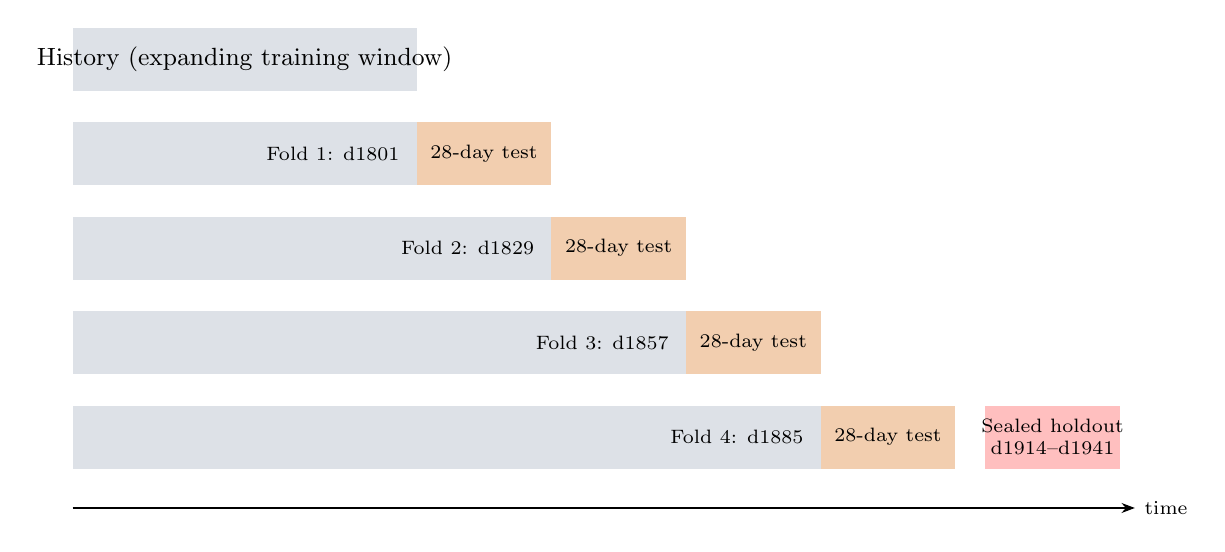
\begin{tikzpicture}[x=0.95cm,y=1cm,>=Stealth]
  \fill[navy!15] (0,0) rectangle (4.6,0.8);
  \node[font=\small] at (2.3,0.4) {History (expanding training window)};
  \foreach \i/\x/\lab in {0/4.6/{Fold 1: d1801},1/6.4/{Fold 2: d1829},2/8.2/{Fold 3: d1857},3/10.0/{Fold 4: d1885}} {
    \fill[accent!35] (\x,-1.2*\i-1.2) rectangle (\x+1.8,-1.2*\i-0.4);
    \fill[navy!15] (0,-1.2*\i-1.2) rectangle (\x,-1.2*\i-0.4);
    \node[font=\scriptsize] at (\x+0.9,-1.2*\i-0.8) {28-day test};
    \node[font=\scriptsize,anchor=east] at (\x-0.1,-1.2*\i-0.8) {\lab};
  }
  \fill[red!25] (12.2,-4.8) rectangle (14,-4.0);
  \node[font=\scriptsize,align=center] at (13.1,-4.4) {Sealed holdout\\d1914--d1941};
  \draw[->] (0,-5.3) -- (14.2,-5.3) node[right,font=\scriptsize] {time};
\end{tikzpicture}
\caption{Expanding-window rolling-origin backtest. Each origin forecasts the next 28 days; the final competition window is never touched.}
\label{fig:timeline}
\end{figure}

\begin{table}[H]
\centering
\caption{Backtest folds.}
\label{tab:folds}
\small
\renewcommand{\arraystretch}{1.2}
\begin{tabular}{@{}l l l r@{}}
\toprule
\textbf{Fold} & \textbf{Origin} & \textbf{Test window} & \textbf{Forecasts}\\
\midrule
1 & \code{d1801} & 2016-01-04 to 2016-01-31 & 6,720\\
2 & \code{d1829} & 2016-02-01 to 2016-02-28 & 6,720\\
3 & \code{d1857} & 2016-02-29 to 2016-03-27 & 6,720\\
4 & \code{d1885} & 2016-03-28 to 2016-04-24 & 6,720\\
\bottomrule
\end{tabular}
\end{table}

\subsection{Evaluation Metrics}
With $M$ evaluated points:
\begin{align}
  \mathrm{MAE} &= \frac1M\sum_i |y_i-\hat y_i|, &
  \mathrm{RMSE} &= \sqrt{\frac1M\sum_i (y_i-\hat y_i)^2},\\
  \mathrm{WAPE} &= \frac{\sum_i |y_i-\hat y_i|}{\sum_i y_i}, &
  \mathrm{PL}_\tau &= \max\!\big(\tau(y-\hat q_\tau),\,(1-\tau)(\hat q_\tau-y)\big).
\end{align}
The empirical coverage $\mathrm{PICP}_{80}$ is the share of actuals falling in $[\hat q_{0.10},\hat q_{0.90}]$, with a nominal value of 80\%. Pinball loss and coverage are reported only for the Kalman models, which produce predictive quantiles.

% ---------------------------- 6. RESULTS ------------------------------
\section{Results}

\subsection{Pooled Point-Forecast Accuracy}
Table~\ref{tab:point} and Figure~\ref{fig:overview} summarise pooled accuracy over all 26,880 predictions.

\begin{table}[H]
\centering
\caption{Point-forecast accuracy across all folds (26,880 series-days). Best value per column in green.}
\label{tab:point}
\small
\renewcommand{\arraystretch}{1.2}
\begin{tabular}{@{}l l c c c@{}}
\toprule
\textbf{Model} & \textbf{Paradigm} & \textbf{MAE} $\downarrow$ & \textbf{RMSE} $\downarrow$ & \textbf{WAPE} $\downarrow$\\
\midrule
LightGBM (global)        & Global tabular GBDT & \best{0.9227} & 2.1081 & \best{0.7640}\\
Kalman LL Seasonal       & Local state-space   & 1.0007 & \best{2.0535} & 0.8286\\
Kalman LT Seasonal       & Local state-space   & 1.0030 & 2.0576 & 0.8305\\
Kalman Local Level       & Local state-space   & 1.0106 & 2.0613 & 0.8368\\
Kalman Single-SKU (M6)   & Local state-space   & 1.0115 & 2.0776 & 0.8375\\
Kalman Local Trend       & Local state-space   & 1.0225 & 2.0976 & 0.8466\\
Naive Weekly Seasonal    & Heuristic baseline  & 1.1869 & 2.5487 & 0.9828\\
Naive Last Value         & Heuristic baseline  & 1.2479 & 2.5151 & 1.0332\\
\bottomrule
\end{tabular}
\end{table}

\begin{figure}[H]
\centering
\includegraphics[width=\textwidth]{figures/metrics_overview.png}
\caption{MAE, RMSE and WAPE for all eight models (LL = local level, LT = local trend). LightGBM (green) leads on MAE and WAPE; the seasonal local-level Kalman model leads on RMSE.}
\label{fig:overview}
\end{figure}

\begin{keybox}[title=Main observations]
\begin{itemize}[leftmargin=1.4em,itemsep=2pt]
  \item \textbf{Point accuracy:} LightGBM reduces MAE by 7.8\% relative to the best Kalman model (1.0007) and by 22.3\% relative to the best naive baseline, weekly seasonal (1.1869); against the last-value baseline the reduction is 26.1\%.
  \item \textbf{Squared error:} the seasonal local-level Kalman model has the lowest RMSE (2.0535 vs.\ 2.1081 for LightGBM). RMSE penalises large errors heavily, so this suggests the Kalman forecasts make fewer large misses on high-demand days, although the pooled results alone do not prove the cause.
  \item \textbf{Trend states do not help:} the local-trend model has the worst Kalman WAPE (0.8466). Retail demand oscillates around a level rather than drifting steadily, so a trend component adds variance without benefit.
\end{itemize}
\end{keybox}

\subsection{Comparison of the Kalman Variants}
The five Kalman variants are close in pooled WAPE (0.8286--0.8466, Figure~\ref{fig:kwape}): adding weekly seasonality helps slightly (local level 0.8368 $\rightarrow$ 0.8286), whereas adding a damped trend hurts (0.8466). The differences are small compared with the gap to LightGBM or to the naive baselines.

\begin{figure}[H]
\centering
\includegraphics[width=0.88\textwidth]{figures/kalman_wape.png}
\caption{Development WAPE of the five Kalman variants. The bars are nearly equal in height; the seasonal local-level model is marginally lowest.}
\label{fig:kwape}
\end{figure}

\subsection{Probabilistic Forecasts: Pinball Loss and Coverage}
Only the Kalman models produce predictive intervals. Table~\ref{tab:prob} and Figures~\ref{fig:cov}--\ref{fig:pinball} show that every variant covers at least the nominal 80\%. The single-SKU model is closest to nominal (81.08\%), whereas the other four variants over-cover at roughly 85--86\%, i.e.\ their intervals are somewhat conservative (wider than necessary). For safety-stock purposes, over-coverage errs on the side of protection but implies extra holding cost.

\begin{table}[H]
\centering
\caption{Probabilistic metrics for the Kalman models. Best value per column in green.}
\label{tab:prob}
\small
\renewcommand{\arraystretch}{1.2}
\begin{tabular}{@{}l c c c c@{}}
\toprule
\textbf{Model} & \textbf{PL Q10} $\downarrow$ & \textbf{PL Q50} $\downarrow$ & \textbf{PL Q90} $\downarrow$ & \textbf{80\% coverage}\\
\midrule
Kalman LL Seasonal     & 0.1318 & \best{0.5004} & 0.3306 & 85.72\%\\
Kalman LT Seasonal     & 0.1347 & 0.5015 & \best{0.3304} & 85.43\%\\
Kalman Local Level     & \best{0.1315} & 0.5053 & 0.3366 & 85.64\%\\
Kalman Single-SKU (M6) & 0.1426 & 0.5058 & 0.3518 & \best{81.08\%}\\
Kalman Local Trend     & 0.1419 & 0.5112 & 0.3371 & 85.37\%\\
\bottomrule
\end{tabular}
\end{table}

\begin{figure}[H]
\centering
\begin{subfigure}[t]{0.49\textwidth}
  \centering\includegraphics[width=\textwidth]{figures/coverage.png}
  \caption{Empirical coverage of the nominal 80\% interval.}\label{fig:cov}
\end{subfigure}\hfill
\begin{subfigure}[t]{0.49\textwidth}
  \centering\includegraphics[width=\textwidth]{figures/pinball.png}
  \caption{Pinball loss at the 10th, 50th and 90th percentiles.}\label{fig:pinball}
\end{subfigure}
\caption{Probabilistic performance of the Kalman variants (LL = local level, LT = local trend).}
\end{figure}

\subsection{Performance by Volume Band}
Table~\ref{tab:band} reports the best Kalman model (local level + seasonal) by volume band. The cohort is balanced (8,960 observations per band), yet relative error rises sharply as volume falls: WAPE is 0.7166 for high-volume series but exceeds 1.0 for medium (1.1136) and low volume (1.2740), because the denominator $\sum y_i$ is tiny when most days are zero. MAE moves the opposite way (1.9453 $\rightarrow$ 0.3566) because absolute demand is lower.

\begin{table}[H]
\centering
\caption{Kalman local level + seasonal by volume band.}
\label{tab:band}
\small
\renewcommand{\arraystretch}{1.2}
\begin{tabular}{@{}l r c c c@{}}
\toprule
\textbf{Volume band} & \textbf{Observations} & \textbf{MAE} $\downarrow$ & \textbf{RMSE} $\downarrow$ & \textbf{WAPE} $\downarrow$\\
\midrule
High   & 8,960 & 1.9453 & 3.3110 & 0.7166\\
Medium & 8,960 & 0.7002 & 1.1062 & 1.1136\\
Low    & 8,960 & 0.3566 & 0.6813 & 1.2740\\
\bottomrule
\end{tabular}
\end{table}

\begin{figure}[H]
\centering
\includegraphics[width=0.82\textwidth]{figures/band_metrics.png}
\caption{Kalman local level + seasonal: WAPE (left; dashed line marks WAPE $=1$) and MAE (right) by volume band.}
\label{fig:band}
\end{figure}

\subsection{Fold-by-Fold Stability}
Table~\ref{tab:foldmae} and Figure~\ref{fig:foldmae} show that the ranking is the same in every fold: LightGBM is best, followed by Kalman LL seasonal, then the naive weekly seasonal and naive last-value baselines. Every model records its highest MAE in the final fold (origin \code{d1885}), although LightGBM stays below 1.0 throughout (0.8821--0.9679) and the last-value baseline barely changes after fold~1 (1.2314--1.2564). No single fold drives the conclusions.

\begin{table}[H]
\centering
\caption{MAE across the four rolling folds. Best per fold in green.}
\label{tab:foldmae}
\small
\renewcommand{\arraystretch}{1.2}
\begin{tabular}{@{}l c c c c@{}}
\toprule
\textbf{Model} & \textbf{Fold 1801} & \textbf{Fold 1829} & \textbf{Fold 1857} & \textbf{Fold 1885}\\
\midrule
LightGBM              & \best{0.8821} & \best{0.9306} & \best{0.9103} & \best{0.9679}\\
Kalman LL Seasonal    & 0.9723 & 1.0145 & 0.9903 & 1.0257\\
Naive Weekly Seasonal & 1.1460 & 1.1835 & 1.1676 & 1.2507\\
Naive Last Value      & 1.2314 & 1.2528 & 1.2509 & 1.2564\\
\bottomrule
\end{tabular}
\end{table}

\begin{figure}[H]
\centering
\includegraphics[width=0.7\textwidth]{figures/mae_by_fold.png}
\caption{MAE by forecast origin. LightGBM is best at every origin; all models find the last fold hardest.}
\label{fig:foldmae}
\end{figure}

\subsection{Naive Baselines Across Origins}
Figure~\ref{fig:naive} shows the pooled WAPE of the two heuristics on the development origins. The weekly seasonal baseline is at or below the last-value baseline at every origin (roughly 0.97--1.00 vs.\ 0.99--1.07), confirming that the 7-day cycle carries real signal. Both hover around a WAPE of 1.0, meaning that a naive forecast is barely better than predicting nothing at all --- the bar that the learned models must clear.

\begin{figure}[H]
\centering
\includegraphics[width=0.82\textwidth]{figures/naive_by_origin.png}
\caption{Pooled WAPE of the naive baselines by development origin.}
\label{fig:naive}
\end{figure}

\subsection{Qualitative Forecast Examples}
We inspect one representative series per volume band. Figure~\ref{fig:naivequal} shows the naive forecasts at origin \code{d1801}. For the high-volume series \code{FOODS_1_004__TX_2} the last-value baseline stays flat at 1 unit while actual sales climb in mid-January with spikes up to 13 units, so both baselines miss the peaks by a wide margin; the weekly seasonal baseline reproduces a repeating pattern that does not match the realised timing. For the low-volume series \code{FOODS_1_038__WI_2} sales are sporadic 0/1 events, and flat or periodic forecasts cannot anticipate which days will be non-zero. The medium-volume example \code{FOODS_1_026__CA_2} is all zeros in this window, so every baseline is trivially correct there --- a reminder of how heavily zeros dominate this cohort.

\begin{figure}[p]
\centering
\begin{subfigure}[t]{0.92\textwidth}
  \centering\includegraphics[width=\textwidth]{figures/cmp_high.png}
  \caption{High volume.}
\end{subfigure}\\[4pt]
\begin{subfigure}[t]{0.92\textwidth}
  \centering\includegraphics[width=\textwidth]{figures/cmp_low.png}
  \caption{Low volume.}
\end{subfigure}\\[4pt]
\begin{subfigure}[t]{0.92\textwidth}
  \centering\includegraphics[width=\textwidth]{figures/cmp_medium.png}
  \caption{Medium volume.}
\end{subfigure}
\caption{Naive baselines (last value and weekly seasonal) versus actual sales at origin \code{d1801}, one series per volume band.}
\label{fig:naivequal}
\end{figure}

Figure~\ref{fig:kalmanqual} shows the Kalman variants with their $q_{10}$--$q_{90}$ bands at the last origin (\code{d1885}). Three behaviours are visible:
\begin{itemize}[leftmargin=2em,itemsep=2pt]
  \item \textbf{Median forecasts hug zero.} For intermittent series the $q_{50}$ forecast sits near zero; the seasonal variants add a small weekly ripple (e.g.\ peaks around 0.4 units for the low-volume series) while the non-seasonal variants are flat.
  \item \textbf{Bands widen with the horizon,} consistent with $V_h=P_{T|T}+hQ+R$, and reach about 1 unit for the low- and medium-volume series.
  \item \textbf{Wide upper bands after long zero runs.} For the high-volume series the realised sales are zero throughout the window, yet the upper band rises to roughly 3--5 units. The model is uncertain because the series was active earlier in the year; here the interval is conservative, which fits the observed over-coverage in Table~\ref{tab:prob}. For the medium-volume series, the series has no sales history in the plotted training window and then records occasional sales of 1--3 units which the median forecast cannot anticipate, although most fall inside the 80\% band.
\end{itemize}

\begin{figure}[p]
\centering
\begin{subfigure}[t]{0.92\textwidth}
  \centering\includegraphics[width=\textwidth]{figures/kv_high.png}
  \caption{High volume (\code{FOODS_1_004__TX_2}).}
\end{subfigure}\\[4pt]
\begin{subfigure}[t]{0.92\textwidth}
  \centering\includegraphics[width=\textwidth]{figures/kv_low.png}
  \caption{Low volume (\code{FOODS_1_038__WI_2}).}
\end{subfigure}\\[4pt]
\begin{subfigure}[t]{0.92\textwidth}
  \centering\includegraphics[width=\textwidth]{figures/kv_medium.png}
  \caption{Medium volume (\code{FOODS_1_026__CA_2}).}
\end{subfigure}
\caption{Kalman variants at origin \code{d1885}: median forecast ($q_{50}$) and 10th--90th percentile band against actual sales.}
\label{fig:kalmanqual}
\end{figure}

% ---------------------------- 7. DISCUSSION ---------------------------
\section{Discussion}

\subsection{Why LightGBM Wins on Point Accuracy}
Global pooling lets the model learn calendar, SNAP, price and lag effects from all 240 series at once, whereas each Kalman filter must infer its parameters from a single, mostly-zero series. The L1 objective also targets the median, which suits zero-heavy data and is consistent with the MAE and WAPE metrics on which LightGBM leads. The paper's working hypothesis is that local maximum-likelihood estimation of $(Q,R)$ becomes unreliable when about 89\% of days are zero (low-volume band); a per-band breakdown for LightGBM would be needed to confirm this directly.

\subsection{Why Kalman Filters Remain Valuable}
\begin{itemize}[leftmargin=2em,itemsep=2pt]
  \item \textbf{Calibrated uncertainty for free:} predictive variance $V_h$ is analytic, and all five variants reach at least the nominal 80\% coverage.
  \item \textbf{Interpretability:} the latent level, trend and seasonal states have direct business meaning.
  \item \textbf{Missing-data handling:} the filter skips updates for unobserved days instead of imputing values.
  \item \textbf{Best RMSE:} the seasonal local-level model gives the lowest squared error of all models.
\end{itemize}

\subsection{Limitations}
\begin{itemize}[leftmargin=2em,itemsep=2pt]
  \item \textbf{Gaussian predictive intervals} are only an approximation for non-negative, count-like, zero-heavy demand; zero-clipping fixes the sign but not the shape of the distribution.
  \item \textbf{Over-coverage} (85--86\%) in four of the five variants shows the intervals are not perfectly calibrated and could be tightened.
  \item \textbf{No probabilistic output for LightGBM} in this phase, so the two paradigms cannot yet be compared on pinball loss or coverage. Quantile-objective LightGBM would address this.
  \item \textbf{Cohort size:} 240 series and four folds are a small sample of the full M5 hierarchy, and the pooled WAPE for low- and medium-volume series exceeds 1.0 for all models.
  \item \textbf{Exogenous variables:} the Kalman variants here use no SNAP, price or event regressors, which LightGBM does.
\end{itemize}

% ---------------------------- 8. PLATFORM -----------------------------
\section{Interactive Diagnostic Platform}
To bridge theory and practice we built a Streamlit application (\code{app.py}) with three components:
\begin{enumerate}[leftmargin=2em,itemsep=2pt]
  \item \textbf{Live Kalman simulation:} sliders for $Q$ and $R$ show the effect on the Kalman gain $K_t$ and on the widening 80\% prediction intervals.
  \item \textbf{Leakage-safe feature explorer:} real-time construction of the 26 tabular features at a chosen forecast origin $T$.
  \item \textbf{Interactive leaderboards:} bar charts and metric sorting across all eight models.
\end{enumerate}

% ---------------------------- 9. CONCLUSION ---------------------------
\section{Conclusion and Operational Recommendations}
Neither local state-space models nor a global tree-based forecaster is a complete solution on its own. Our results support a hybrid policy:
\begin{enumerate}[leftmargin=2em,itemsep=2pt]
  \item \textbf{Procurement baseline:} use global LightGBM for purchase-order sizing, since it has the lowest expected unit error (WAPE 0.7640, MAE 0.9227).
  \item \textbf{Safety-stock sizing:} use the Kalman predictive variance $V_h$ to set dynamic, calibrated safety-stock buffers (81.08\% empirical coverage for the single-SKU model at a nominal 80\%).
\end{enumerate}

\textbf{Phase~2 roadmap.} Future work will combine the two modalities in global probabilistic recurrent architectures such as DeepAR~\cite{salinas2020} and Temporal Fusion Transformers, using Kalman-filtered states as dynamic structural inputs, and will add quantile-based LightGBM so that all models can be compared on probabilistic metrics.

% ---------------------------- REFERENCES ------------------------------
\begin{thebibliography}{9}\small
\bibitem{kalman1960} R.~E. Kalman, ``A new approach to linear filtering and prediction problems,'' \emph{Journal of Basic Engineering}, vol.~82, no.~1, pp.~35--45, 1960.
\bibitem{salinas2020} D.~Salinas, V.~Flunkert, J.~Gasthaus, and T.~Januschowski, ``DeepAR: Probabilistic forecasting with autoregressive recurrent networks,'' \emph{International Journal of Forecasting}, vol.~36, no.~3, pp.~1181--1191, 2020.
\bibitem{harvey1990} A.~C. Harvey, \emph{Forecasting, Structural Time Series Models and the Kalman Filter}. Cambridge University Press, 1990.
\bibitem{ke2017} G.~Ke \emph{et al.}, ``LightGBM: A highly efficient gradient boosting decision tree,'' in \emph{Advances in Neural Information Processing Systems (NeurIPS)}, vol.~30, 2017.
\bibitem{makridakis2022} S.~Makridakis, E.~Spiliotis, and V.~Assimakopoulos, ``The M5 accuracy competition: Results, findings and conclusions,'' \emph{International Journal of Forecasting}, vol.~38, no.~4, pp.~1346--1364, 2022.
\bibitem{boylan2021} J.~E. Boylan and A.~A. Syntetos, \emph{Intermittent Demand Forecasting: Context, Methods and Applications}. John Wiley \& Sons, 2021.
\end{thebibliography}

\end{document}
